% CHAPTER START
The Trigger/DAQ system sends and saves data from the detector to a persistent data storage solution.
It's at this stage where the data isn't yet ready for an effective analysis, so what needs to happen is the data needs to be reconstructed and consolidated into physics objects, or Analysis Object Data (AOD) files.
Creating AODs from data requires significant computation power and Athena is the software framework that plays a significant role in this process.
This chapter will cover some of the important software tools used by ATLAS to run derivation jobs, as well as introduce data structures that represent event information. 

\section{Athena and ROOT}
% \subsection{What is Athena}
Athena is the open-source software framework for the ATLAS experiment.\cite{athena}
It uses on other software such as ROOT, Geant4 and other software as part of the LCG software stack. 
It also provides some in-house based analysis tools as well as tools for specifically ROOT based analysis.

% % CMake
CMake and Make are open-source software that is used to build Athena, ROOT, and other software.
A sparse build is a way to make changes to an individual package of code without having to recompile the entire framework at once, which saves time and resources. 
A user can create a text file identifying the path to the package modified, and the sparse build for Athena will proceed upon issuing the following commands:
\begin{lstlisting}[language=bash]
    cmake -DATLAS_PACKAGE_FILTER_FILE=../package_filters.txt ../athena/Projects/WorkDir/ 
    make -j
\end{lstlisting}
Where \verb|../package_filters.txt| is the text file containing the path to the package modified, and \verb|../athena/Projects/WorkDir/| is the path to the Athena source.

% How we used it
% % Athena POOL
AthenaPOOL is data storage architecture suite of packages within Athena that provide conversion services. 
It originated as a separate project to serve as a layer between the transient data, stored in memory, used by the software framework and the data stored permanently, or persistently.
The transient/persistent style of representing event data will be further explained in Section \ref{sec:IO_EDM}.


% % Component Accumulator
An important step throughout the development of Athena is to ensure any new changes to the codebase won't overrule the functionality of core features to the present workflows.
One of the areas needed to be tested before and upon merging of any new changes to Athena is the I/O functionality, or the performance of reading and writing of stored objects within a broader context of various jobs, i.e. reconstruction or derivation.
These are unit tests which are scripts written in Python and call upon algorithms written in C++. 
The python scripts are used to set the job options for the algorithms added to the component accumulator (CA), job options like flag definitions, input and output file names, and other algorithm specific options.
While CA is a more general mechanism to run any kind of job with Athena, it's within the scope of this thesis where the focus is on testing core I/O functionality of the new event data model. 
A general CA script written in pseudocode would take the form: 
\begin{lstlisting}[language=Python]
    # Import Packages
    from AthenaConfiguration.AllConfigFlags import initConfigFlags
    from AthenaConfiguration.ComponentFactory import CompFactory
    from OutputStreamAthenaPool.OutputStreamConfig import OutputStreamCfg, outputStreamName

    # Set Job Options
    outputStreamName = "StreamA"
    outputFileName = "output.root"

    # Setup flags
    flags = initConfigFlags()
    flags.Input.Files = ["input.root"]
    flags.addFlag(f"Output.{streamName}FileName", outputFileName)
    # Other flags
    flags.lock()

    # Main services
    from AthenaConfiguration.MainServicesConfig import MainServicesCfg
    acc = MainServicesCfg( flags )

    # Add algorithms
    acc.addEventAlgo( CompFactory.MyAlgorithm(MyParameters) )

    # Run
    import sys
    sc = acc.run(flags.Exec.MaxEvents)
    sys.exit(sc.isFailure())
\end{lstlisting}


% What is ROOT
ROOT is an open-source software framework used for high-energy physics analysis at CERN.\cite{ROOT_about} 
It uses C++ objects to save, access, and process data brought in by the various experiments based at the LHC, the ATLAS experiment uses it in conjunction with Athena.
ROOT largely revolves around organization and manipulation of TFiles and TTrees into ROOT files.
A TTree represents a columnar dataset, and the list of columns are called branches. 
The branches have memory buffers that are automatically allocated by ROOT. 
These memory buffers are divided into corresponding baskets, whose size is designated during memory allocation.
More detail on branch baskets are explored in Chapter \ref{chap:Toy_Model} and \ref{chap:DAODProd}.

% What we looked at/How we used it

\subsection{Continuous Integration (CI) and Development}
CI is a software development practice where new code is tested and validated upon each merge to the main branch of a repository. 
Every commit to the main branch is automatically built and tested for specific core features that are required to work with the codebase. 
This helps to ensure that the codebase is working as intended and that the new code is compatible with the existing codebase.

Athena is hosted on GitLab and developed using CI with an instance of Jenkins, called ATLAS Robot, which builds and tests the new changes within a merge request interface. 
ATLAS Robot will then provide a report of the build and test results.
If the build or test fail, ATLAS Robot will provide a report of which steps failed and why.
This allows for early detection of issues before the nightly build is compiled and tested.



\section{TTree Object} \label{section: ATLASIO_TTreeObject}
A TTree is a ROOT object that organizes physically distinct types of event data into branches.
Branches hold data into dedicated contiguous memory buffers, and those memory buffers, upon compression, become baskets.
These baskets can have a limited size and a set minimum number of entries. 
The Athena default basket size at present is 128 kB, and the default minimum number of entries is 10. 

One function relevant to TTree is \verb|Fill()|. 
\verb|Fill()| will loop over all of the branches in the TTree and compresses the baskets that make up the branch.
This removes the basket from memory as it is then compressed and written to disk.
It makes reading back branches faster as all of the baskets are stored near each other on the same disk region. \cite{ROOT_TTree}

% AutoFlush
\verb|AutoFlush| is a function that tells the \verb|Fill()| function after a designated number of entries of the branch, in this case vectors, to flush all branch buffers from memory and save them to disk. 


\section{Derivation Production Jobs}
 \label{section: ATLASIO_Derivation}

A derivation production job takes AODs, which comes from the reconstruction step at $\mathcal{O}(1 \text{ MB})$ per event, and creates a derived AOD (DAOD) which sits at $\mathcal{O}(10 \text{ kB})$ per event.
Derivation production is a necessary step to make all data accessible for physicists doing analysis as well as reducing the amount of data that needs to be processed.
While derivations are reduced AODs, they often contain additional information useful for analysis, such as jet collections and high-level discriminants.\cite{PHYSLITE_A_new_2024}
The two mainstream output file formats Athena is capable of handling are PHYS and PHYSLITE.  
Figure \ref{fig:IO_tt_PHYS_vs_PHYSLITE} shows the object composition of a PHYS and PHYSLITE $t\bar{t}$ sample. 
\begin{figure}[h]
    \centering
    \begin{subfigure}{.5\textwidth}
        \centering
        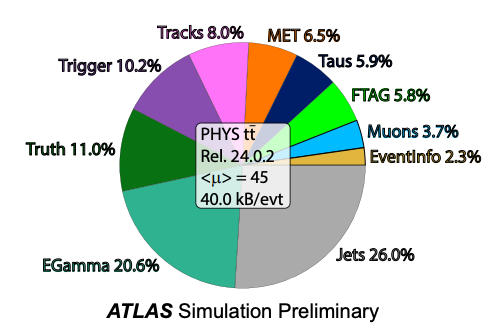
\includegraphics[width=\textwidth]{content/img/tt_PHYS.png}
        % \caption{A subfigure}
        \label{fig:IO_tt_PHYS_subA}
      \end{subfigure}%     
      \begin{subfigure}{.5\textwidth}
        \centering
        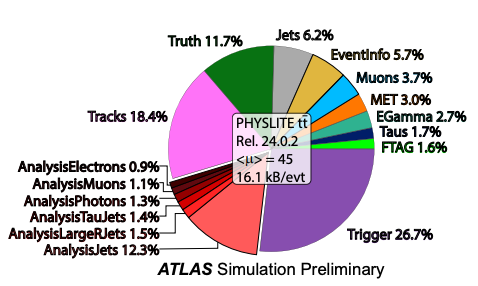
\includegraphics[width=\textwidth]{content/img/tt_PHYSLITE.png}
        % \caption{B subfigure}
        \label{fig:IO_tt_PHYSLITE_subB}
      \end{subfigure}% 
    \caption{Object composition of a PHYS and PHYSLITE $t\bar{t}$ sample from Run 3.}
    \label{fig:IO_tt_PHYS_vs_PHYSLITE}
\end{figure}
PHYS output files, at 40.0 kB per event, is predominantly made of jet collections, while PHYSLITE, at 16.1 kB per event, has more trigger and track information.
There is ongoing work to reduce the amount of Trigger information in PHYSLITE which would help further reduce the file size saved to disk.
PHYSLITE, being the smallest file of the two, sees the largest effect upon attempts of optimization. 
These jobs can demand heavy resource usage on the GRID, so optimization of the AOD/DAODs for derivation jobs can be vital. 

\begin{figure}[h]
    \centering
    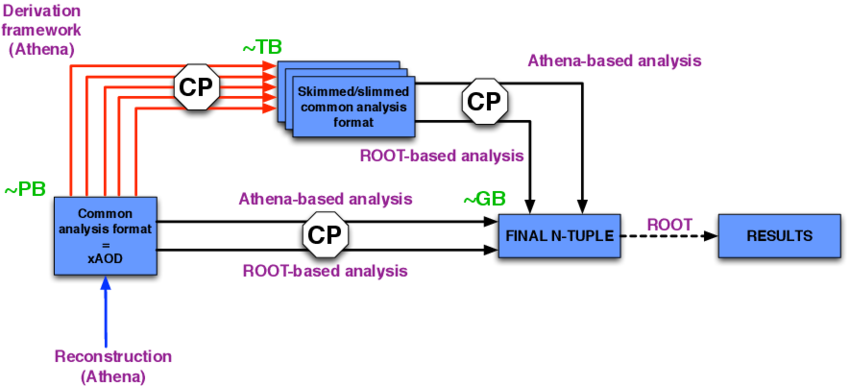
\includegraphics[width=0.8\textwidth]{content/img/catmore-derivation.png}
    \caption{Derivation production from Reconstruction to Final N-Tuple\cite{DAOD_Laycock_2014}}
    \label{fig:IO_derivation_framework}
\end{figure}

The derivation framework is sequence of steps that are performed on the AODs to create the DAODs.
Skimming is the first step in the derivation framework, and it's responsible for removing whole events based on pre-defined criteria.
Thinning is the second step, and it removes whole objects based on pre-defined criteria.
Lastly slimming removes variables from objects uniformly across events. 


\section{Event Data Models} \label{sec:IO_EDM}
% \subsection{What is an Event Data Model}
An Event Data Model (EDM) is a collection of classes and their relationships to each other that provide a representation of an event detected with the goal of making it easier to use and manipulate by developers.
An EDM is how particles and jets are represented in memory, stored to disk, and manipulated in analysis.
It's useful to have an EDM because it brings a commonality to the code, which is useful when developers reside in different groups with various backgrounds.
An EDM allows those developers to more easily debug and communicate issues when they arise.  

\subsection{Transient/Persistent (T/P) EDM}
One of the previous EDM schemas used by ATLAS concerned a dual transient/persistent status of AOD.
With this EDM, the AOD was converted into an ntuple based format called D3PDs. 
While this conversion allowed for fast readability and partial read for efficient analysis in ROOT, it left the files disconnected from the reconstruction tools found in Athena.\cite{Athena_xAOD_design}
When transient data was present in memory, it could have information attached to the object and gain in complexity the more it was used.
Transient data needed to be simplified before it could become persistent into long-term storage (sent to disk). 
ROOT had trouble handling the complex inheritance models that would come up the more developers used this EDM. 
Before the successor to the T/P EDM was created, ATLAS physicists would convert data samples using the full EDM to a simpler one that would be directly readable by ROOT.
This would lead to duplication of data and made it challenging to develop and maintain the analysis tools to be used on both the full EDM and the reduced ones.
Additionally, converting from transient to persistent data was an excessive step which was eventually removed by the adoption of using an EDM that blends the two stages of data together, this was dubbed the xAOD EDM.




\subsection{xAOD EDM}
The xAOD EDM is the successor to the T/P EDM and brings a number of improvements.
This EDM, unlike T/P, is usable both on Athena and ROOT.
It's easier to pick up for analysis and reconstruction. 
The xAOD EDM has the ability to add and remove variables within an \verb|ItemList| at runtime, specified in the CA script, these variables are ``decorations."

The xAOD EDM use two types of objects handle data, interface objects and payload objects. 
Interfaces act as an interface for the user to access the object but without its stored data. 
This differs from T/P where the user would have to load an object into memory to access the object. 
If the user wanted to delay the loading of data into memory, they could use the interface object to do so. 
The payload object contains the data for the interface object and is allocating contiguous blocks of memory. 
Payload classes are often referred to as auxiliary storage. 

The specific data structure used by ATLAS is the ROOT TTree, but the EDM is agnostic to the type of data structure used. 
ATLAS specific libraries are not required to handle files written in the xAOD format since the payload can be read directly from the contiguous allocation of memory, a central tenent of the xAOD EDM.
This allows for the separation of ATLAS specific analysis frameworks and the preferred analysis tool of the user.
More information on how the xAOD EDM is deployed into unit tests in Section \ref{sec:Mod_utests_xAOD_object}.

